\PassOptionsToPackage{hyphens}{url}
\documentclass[compress,aspectratio=169]{beamer}

\usetheme{Reading}

\graphicspath{{fig/}{img/}{../logo/}}

\newcommand{\ok}[1]{{#1 (done)}}
\newcommand{\ongoing}[1]{{#1 (ongoing)}}
\newcommand{\started}[1]{{#1 (started)}}
\newcommand{\pending}[1]{{#1 (pending in plan)}}
\newcommand{\hrefb}[2]{\href{#1}{\textcolor{blue}{#2}}}

\subtitle{}
\title{\huge The HPC Certification Program}
\author{J. Kunkel on behalf of the HPC Certification Forum}
\date{2019-06-18}
\authorURL{https://hpc-certification.org}
\authorFooter{Julian M. Kunkel}
\venue{HPC-SIG meeting}
\institute{Department of Computer Science}
\groupLogo{
\includegraphics[width=2.5cm]{hpccf-small}}
\titleLogo{ 
\includegraphics[height=2.5cm]{blur-book-stack-books-590493}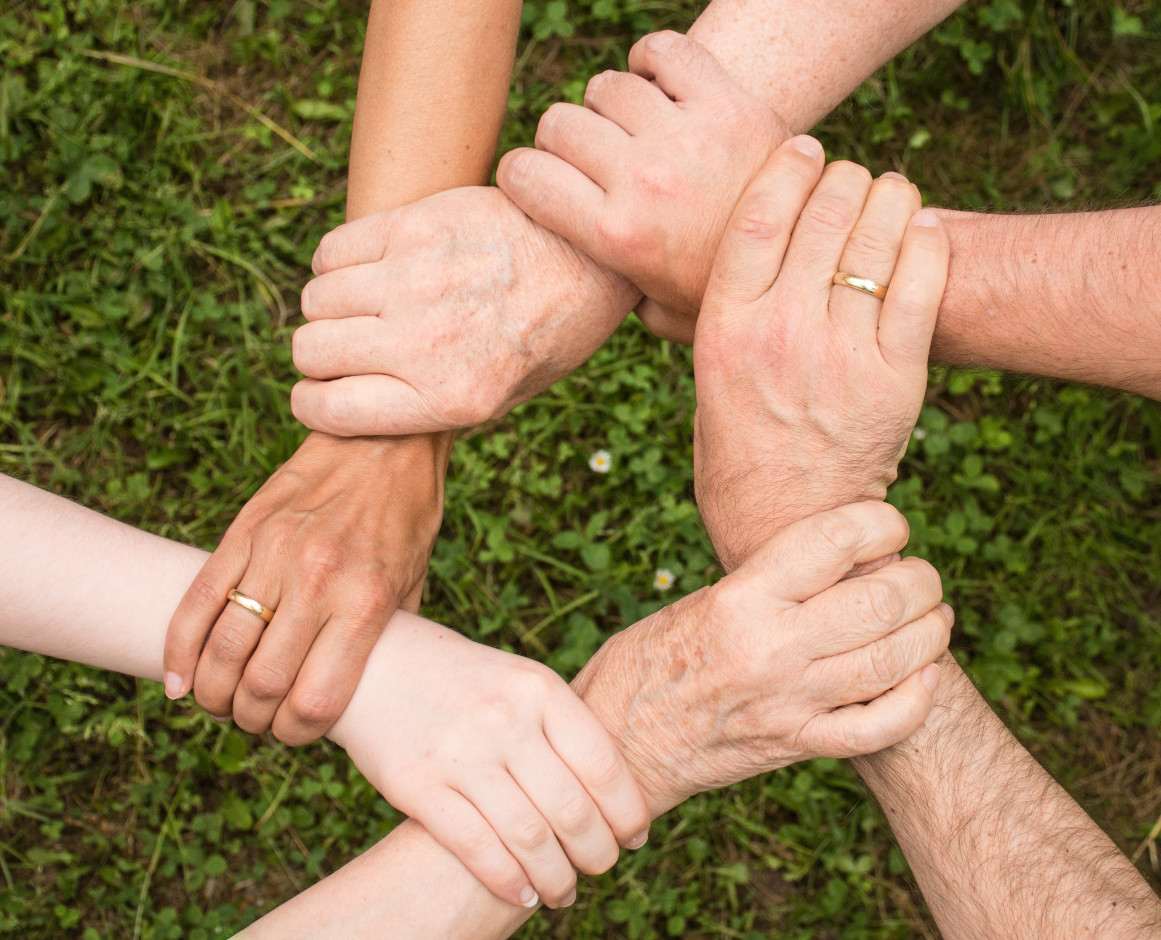
\includegraphics[height=2.5cm]{ground-group-growth-461049}
\includegraphics[height=2.5cm]{accomplishment-ceremony-college-267885}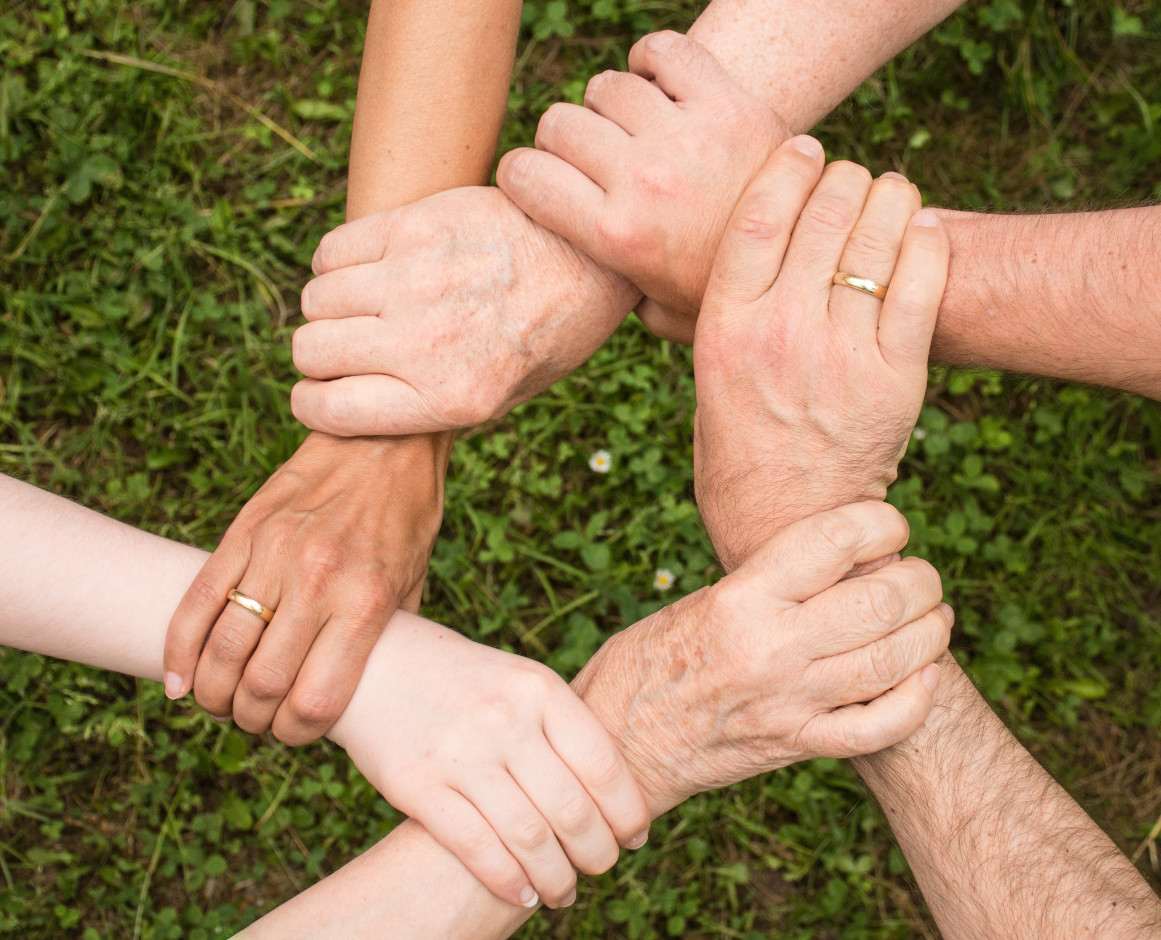
\includegraphics[height=2.5cm]{ground-group-growth-461049}
\includegraphics[height=2.5cm]{blur-book-stack-books-2}}


\begin{document}

\begin{frame}[plain]{}
	\maketitle
	{\fontsize{5.85pt}{6pt}\selectfont PeCoH is supported by Deutsche Forschungsgemeinschaft (DFG) under grants LU 1335/12-1, OL 241/2-1, RI 1068/7-1}
\end{frame}


\begin{frame}{The HPC Certification BoF: Agenda}
	\begin{block}{Short presentations}
	\begin{itemize}
		\item Introduction to the HPC Certification Program
		\item HPC tools and usage: a view from the community
		\item Skill tree introduction
		\item Certification process introduction
	\end{itemize}
	\end{block}

	\begin{block}{Community discussion}
		We prepared several stations in the room allowing you to give feedback % Details later
	\end{block}

	\begin{block}{Wrapup: Summary \& Conclusion}
		\begin{itemize}
			\item Roadmap
			\item Joint discussion
		\end{itemize}
	\end{block}

\end{frame}


\section{The Program}
\sectionIntroHidden

\subsection{}

\begin{frame}{HPC Certification Program}
	\begin{block}{Motivation}
		\begin{itemize}

			\item Not all users possess the right level of training
				\begin{itemize}
				\item Inefficient usage of systems, frustration, lost potential
				\item Good training saves compute time and costs!
				\end{itemize}
			\item Learning is not easy
			\begin{itemize}
				\item Users need to understand beneficial knowledge for tasks
				\item There exist various different training material
				\item Teaching of different data centers is hard to compare
			\end{itemize}
			\item Data center have difficulties to verify the skills of users
		\end{itemize}
	\end{block}

\end{frame}



\begin{frame}{The HPC Certification Program}
		\begin{block}{Goals}
			\begin{itemize}
				\item Standardizing HPC knowledge representation
          \begin{itemize}
						\item What competences exist, how are they defined?
            \item Supporting navigation and role-specific knowledge maps
          \end{itemize}
				\item Establishing international certificates attesting knowledge
			\end{itemize}
		\end{block}

		\begin{block}{Important!}
			\begin{itemize}
				\item We do not compete with content providers
				\item We do not intent to create a curriculum
			\end{itemize}
		\end{block}
\end{frame}


\begin{frame}{Content of the Certification Program}
	\begin{itemize}
		\item A \textbf{skill} defines background, objectives, learning outcomes
		\item The \textbf{skill tree} organizes the competences as hierarchical skills
		\item Certificates bundle several skills into attestable unit
	\end{itemize}

	\begin{figure}
		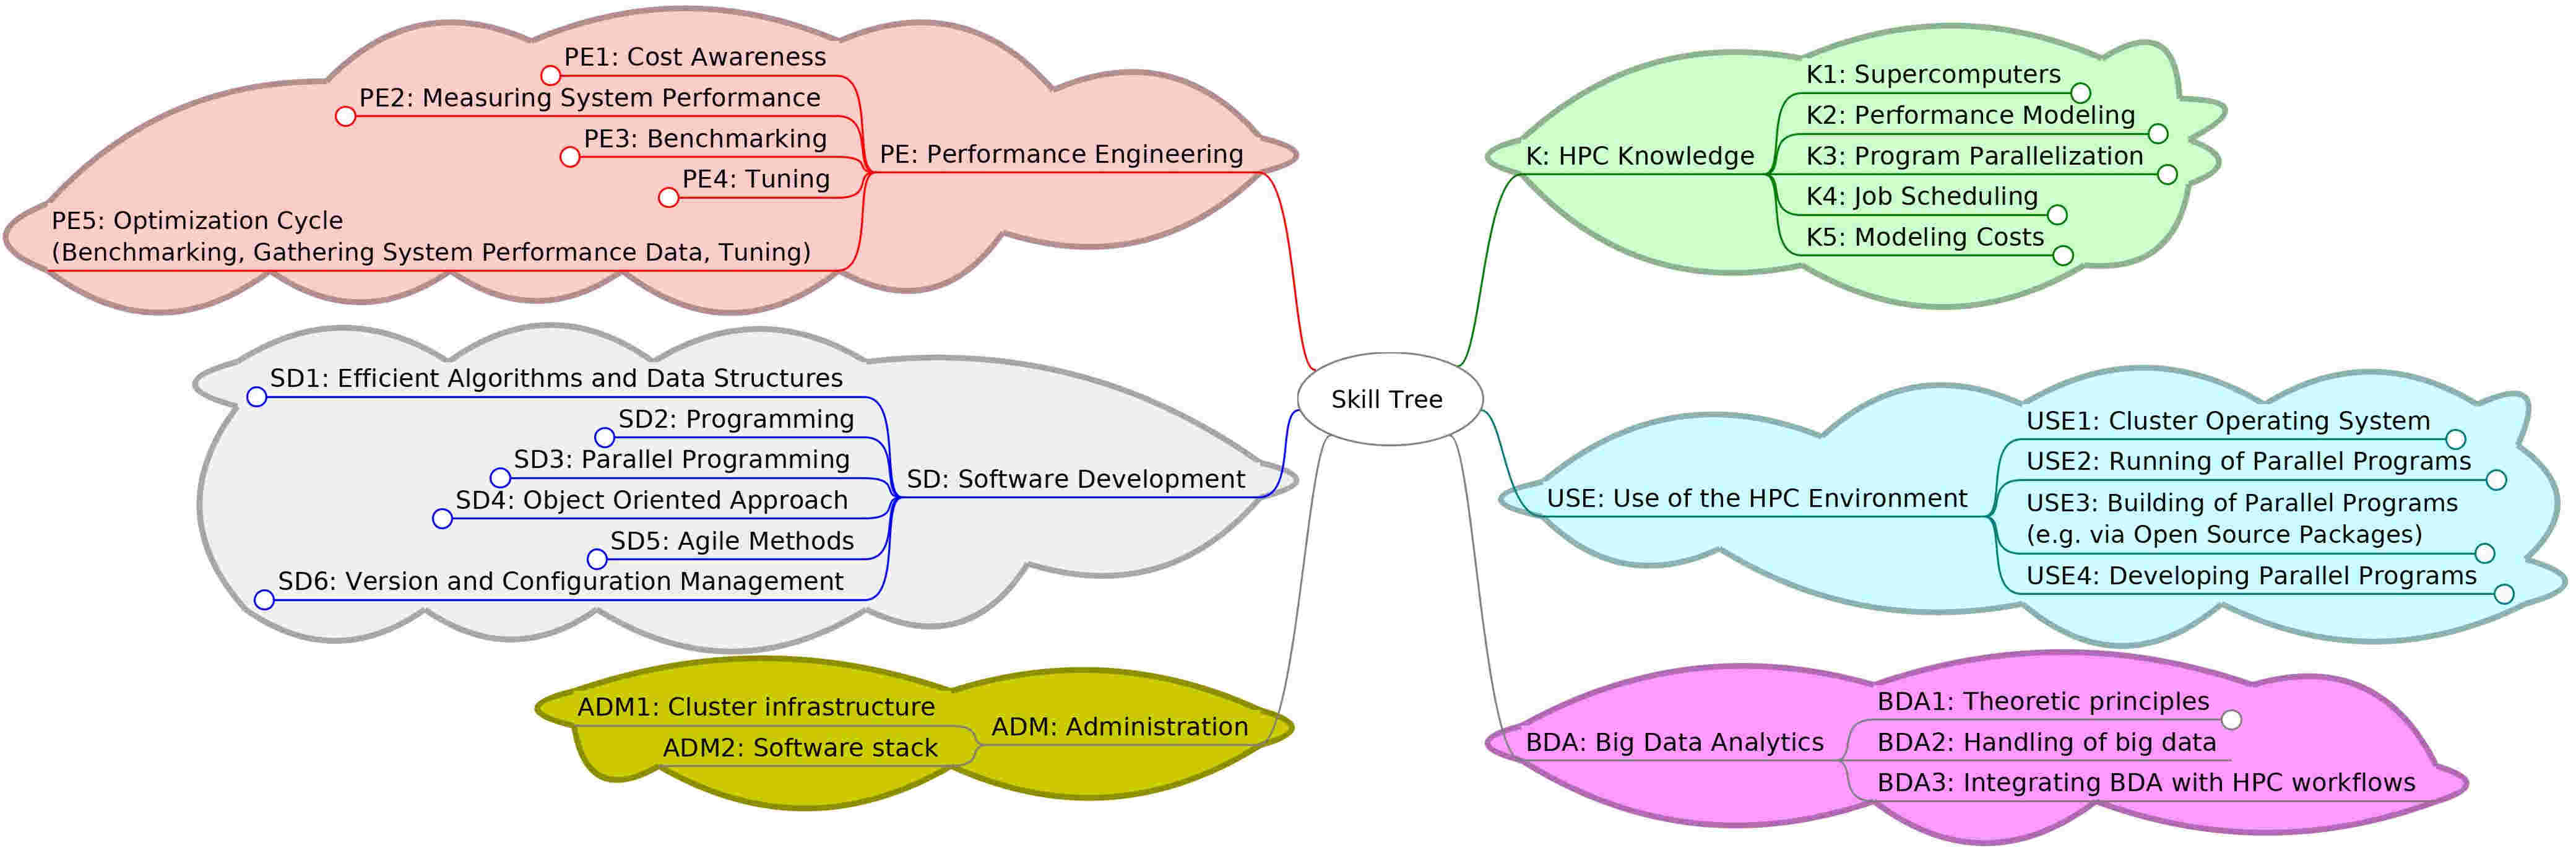
\includegraphics[width=\textwidth]{skill-tree}
		\vspace*{-2em}
		\caption{Top-levels of the skill tree (We are working on ADM and BDA branches)}
	\end{figure}
\end{frame}



\begin{frame}{Classification of HPC Competences}
	\begin{itemize}
		\item Organization of HPC skills
		\begin{itemize}
			\item Skills are typically depending on sub-skills $\Rightarrow$ tree structure
			\item References to skills are possible; still skills are building blocks for various tasks
			\item One skill can have multiple instances for different skill levels
		\end{itemize}

		\item Granularity of skill descriptions
		\begin{itemize}
			\item Too fine $\Rightarrow$ content of a skill is predefined at leaf level
			\item Too coarse $\Rightarrow$ no help for structuring the material
			\item Guiding principle: leaf node should be coverable in 2-4 hour lecture/workshop
		\end{itemize}

		\item External information can be linked to the skills providing different \textbf{views}
		\begin{itemize}
			\item Suitability for a user role (Tester, Builder, Developer)
			\item Suitability for a scientific domain (Chemistry, Physics, ...)
			\item View: purpose-specific representation / coloring / content
				\begin{itemize}
				\item Groups/institutions can derive a new skill tree with their own emphasis
				\item  What should people know to effectively work in your environment?
				\end{itemize}
		\end{itemize}
	\end{itemize}
\end{frame}



\begin{frame}{Further Considerations}
	\begin{itemize}
		\item Certificate definition
		\begin{itemize}
			\item Bundles a set of useful skills together %(e.g. "Getting startet with HPC Clusters")
			\item A users' HPC qualification is certified by successful exams
		\end{itemize}
		\item Separation of skill, certificates and content provider
		\begin{itemize}
			\item Similar to the concept of a high school graduation exam %("Zentralabitur")
			\item Learning material can be provided by different institutions
			\item Teachers can put badges on material: this "trains XYZ"
		\end{itemize}
		\item Verification of skill tree and certification approach
			\begin{itemize}
				\item We utilize the HPC community/practitioners to justify approaches
			\end{itemize}
	\end{itemize}
\end{frame}


\begin{frame}{Status}

\begin{columns}
\column{0.8\textwidth}
	\begin{itemize}
	\item Organizing regular meetings (see our webpage)
	\item Released a first skill tree (we will discuss this after the talks)
	\item Released technical representations of the HPC skills
	\item Released JavaScript for visualization of skill tree \hrefb{https://www.hpc-certification.org/skills/}{(demo)}
		\begin{itemize}
			\item Enables views: adjustable/embedable in your webpage
		\end{itemize}
	\item Developed prototype for exam process: legal framework
	\item Designed seal of endorsement
	\item Engaged with various stakeholders (e.g., SIGHPC Edu)
	\item Conducted survey to verify the skill tree (more to come!)
\end{itemize}

\column{0.2\textwidth}
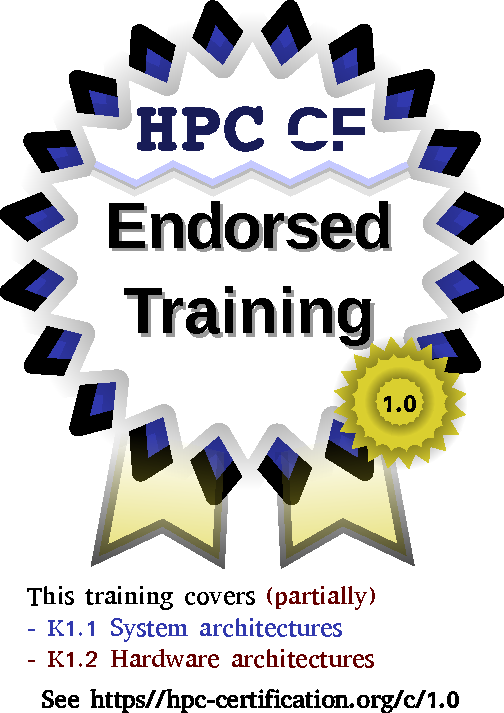
\includegraphics[width=\textwidth]{certified.pdf}
\end{columns}

\medskip

\textit{All our developments are under open licenses (except the exam questions)}
\end{frame}




\section{The HPC Certification Forum}
\sectionIntroHidden

\begin{frame}{The 
\includegraphics[width=0.45\textwidth]{hpccf-full}}
	The HPC-CF is the central authority for the development of the program

	\begin{block}{Organization Details}
		\begin{itemize}
			\item An independent international body
			\item Organized into
				\begin{itemize}
					\item Steering board
					\item Full members with voting rights
					\item Associate members
				\end{itemize}
		\end{itemize}
	\end{block}

	\begin{block}{Responsibilities}
		\begin{itemize}
			\item Curating and maintaining the skill tree and certificates
			\item Providing tools and ecosystem around the competences
		\end{itemize}
	\end{block}
\end{frame}

\begin{frame}{Governance}

	\smallskip
  We have an initial set of governance rules splitting responsibility across roles
  %\vspace*{-1em}

  \begin{block}{Current Chairs}
  \vspace*{-0.5em}
  \begin{itemize}
    \item Program chair: Julian Kunkel (University of Reading)
    \item Curriculum chair: Kai Himstedt (University of Hamburg)
    \item  Topic chairs:
    \begin{itemize}
      \item HPC Knowledge: Lev Lafayette (University of Melbourne)
      \item Performance Engineering: Anja Gerbes (University of Frankfurt)
      \item Use of the HPC Environment: Jean-Thomas Acquaviva (DDN)
      \item Software Development: Waseem Kamleh (University of Adelaide)
			\item Administration: Sharan Kalwani (DataSwing)
			\item Big Data Analytics: Julian Kunkel // Interim
    \end{itemize}
    \item Examination chair: was not seated in 2018
    \item Publicity chair: Weronika Filinger
  \end{itemize}
  \end{block}
\end{frame}

\section{Certification Process}
\sectionIntroHidden

\begin{frame}{Certification: Assessment Prototype}
		\begin{itemize}
			\item[\color{readingRed}{1.}] User takes multiple-choice test online (any time!)
			\begin{itemize}
				\item A combination of JavaScript and a web service
				\item System selects number of questions randomly from a pool
					\begin{itemize}
						\item The questions are managed with rigorous license agreement
					\end{itemize}
				\item System draws 4-5 responses from 10 possible responses (some randomized)
			\end{itemize}
			\item[\color{readingRed}{2.}] Choices are submitted to the web server
			\item[\color{readingRed}{3.}] \textit{Manual approval} of the result
			\item[\color{readingRed}{4.}] Automatic creation of certificate and returned by email
			\begin{itemize}
							\item Permanent computer-verifiable proof that skill is created
							\begin{itemize}
								\item Return a text version with GPG signature
								\item Return a link that can be verified on hpc-certification.org
							\end{itemize}
			\end{itemize}
			\item Privacy: minimize information stored on servers, keep some for statistics
			\item Includes some measure to prevent cheating and brute forcing (e.g., delay)
		\end{itemize}
\end{frame}

\begin{frame}[fragile]{Certification: Certificate}
\begin{columns}
	\column{0.6\textwidth}
	\begin{block}{Text representation}

		\scriptsize
		\begin{verbatim}
-----BEGIN PGP SIGNED MESSAGE-----
Hash: SHA512
HPC Certification Forum Certificate
This text confirms that "Jane Doe" has
successfully obtained the certificate
"HPC driving license" (id: 1) at 02/2019.
Verification URL: https://hpc-certification.org/[...]
-----BEGIN PGP SIGNATURE-----
[...]
-----END PGP SIGNATURE-----
		\end{verbatim}
	\end{block}

\column{0.4\textwidth}
	\begin{block}{Certificate}
		\medskip
		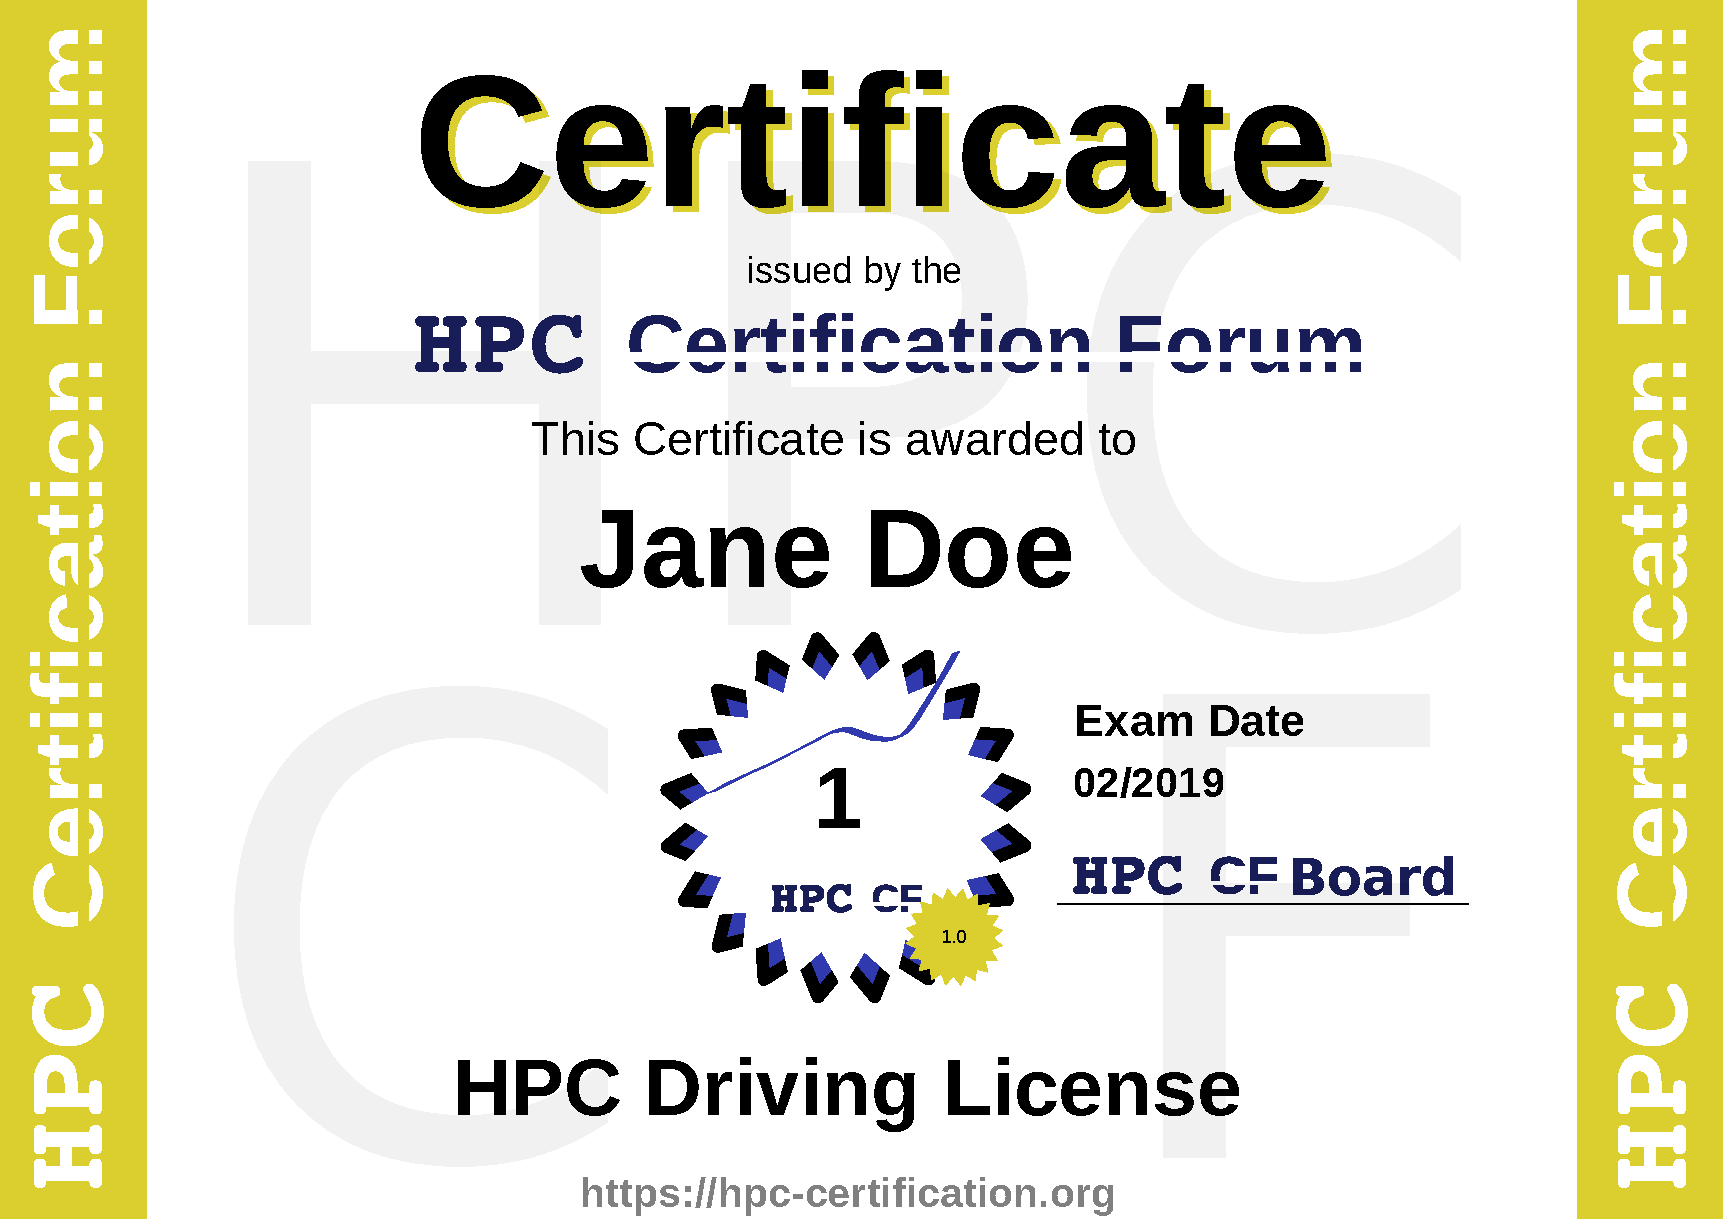
\includegraphics[width=\textwidth]{jane-doe}
	\end{block}
\end{columns}
\end{frame}



\section{Roadmap \& Conclusions}
\sectionIntroHidden


\begin{frame}{Roadmap: Supercomputing 2019}
		\begin{itemize}
			\item Finalizing documentation how to create views with the JavaScript
        \begin{itemize}
          \item This will allow to outsource roles (e.g., tester) but also links to material
        \end{itemize}
      \item Creating converters for markdown version of the skill-tree
			\item Completing the online exam for the certification (of some base courses)
				\begin{itemize}
					\item Determine legal disclaimer / terms of service (help welcome)
				\end{itemize}
      \item Link third-party workshop material (of some base courses)
			\item Discuss affiliation program for institutions/companies
			\item Map out content by the \textit{SIGHPC Education Chapter Content Committee}
		\end{itemize}
  \label{frame:last}
\end{frame}


\begin{frame}{Outlook and Expected Benefits}
	\begin{block}{HPC practitioners}
		\vspace*{-0.2cm}
	\begin{itemize}
	\item Increase motivation to participate as the certificates are recognized in a CV
	\item Validate knowledge via tests
	\item Browse relevant competences
	\item Identify recommended and required skills related to certain tasks
	\item Understand and compare teaching offers across sites
	\end{itemize}
	\end{block}
	\vspace*{-0.3cm}
	\begin{block}{Data centers}
		\vspace*{-0.2cm}
	\begin{itemize}
	\item Increase sharing of teaching materials
	\item Simplifies documentation of taught skills
	\item Identify missing teaching activities
	\item Tailor skill-representation specifically to users
	\item Correlate lack of skills with efficient use
	\end{itemize}
	\end{block}
\end{frame}




\begin{frame}{Summary}

	\begin{block}{HPC Certification Program}
		\begin{itemize}
			\item Effort to standardize representation/certification of relevant HPC skills
      \begin{itemize}
        \item Hierarchical definition of skills for practitioners
        \item Building blocks that can be cherry-picked for different tasks
				\item It's goal is \textbf{NOT} to provide content or a linear curriculum
      \end{itemize}
			\item Perspective for data centers
				\begin{itemize}
					\item Use statistics and machine learning to direct users to right skills
					\item Make certain skills a mandatory requirement?
				\end{itemize}
			\item Customizable representation and navigation for data centers/domains
      \begin{itemize}
        \item Interactive viewer to browse skills and related content
				\item We will use the viewer to link good content to the skills, too!
      \end{itemize}
      \item Visit us and join our Slack/mailing lists: \url{https://hpc-certification.org}
		\end{itemize}
	\end{block}
\end{frame}







\end{document}
